\باب{بنیادی حساب}
	ثنائی نظام میں حساب بالکل اسی طرح کیا جاتا ہے جس طرح اعشاری نظام میں۔چند مثالوں کے مطالعہ سے  وضاحت ہو گی۔
	
	ثنائی نظام میں دو اعداد کا مجموعہ اعشاری نظام میں دو اعداد کے مجموعہ سے سمجھا جا سکتا ہے۔اعشاری نظام کی مندرجہ ذیل مثال پر غور کریں جس میں \عددی{37.5} اور \عددی{29.6}     جمع کیے گئے ہیں۔
\begin{align*}
\begin{split}
&11\\
&37.5\\
+&29.6\\
\noalign{\smallskip}\hline\noalign{\smallskip}
&67.1
\end{split}
\end{align*}
آپ نے دیکھا کہ    حاصل\عددی{(1)}  کو  (بائیں)   زیادہ  وزنی  مقام پر منتقل کیا   گیا۔یہی    ثنائی  جمع   میں کیا جائے گا۔ ثنائی نظام میں صرف دو ہندسے،  \عددی{0} اور \عددی{1}، پائے جاتے ہیں جن  کی چار ممکنہ جمع درج ذیل ہیں۔
\begin{align*}
\begin{split}
1&\\
&1\\
+&1\\
\noalign{\smallskip}\hline\noalign{\smallskip}
1&1
\end{split}&
\begin{split}
&\\
&1\\
+&0\\
\noalign{\smallskip}\hline\noalign{\smallskip}
0&1
\end{split}&
\begin{split}
&\\
&0\\
+&1\\
\noalign{\smallskip}\hline\noalign{\smallskip}
0&1
\end{split}&
\begin{split}
&\\
&0\\
+&0\\
\noalign{\smallskip}\hline\noalign{\smallskip}
0&0
\end{split}
\end{align*}


پہلی تین جمع   میں حاصل  \عددی{0} جبکہ آخری میں حاصل \عددی{1}  ہے۔

آئیں،  زیادہ ثنائی ہندسوں کے اعداد کی  جمع   کی  مثالیں  دیکھیں؛ ان کی  اعشاری نظام میں  جمع  بھی دی گئی ہیں۔
\begin{align*}
\begin{split}
&1\\
&13\\
+&09\\
\noalign{\smallskip}\hline\noalign{\smallskip}
&22_{10}
\end{split}&
\begin{split}
1&\phantom{11}1\\
&1101\\
+&1001\\
\noalign{\smallskip}\hline\noalign{\smallskip}
1&0110_2
\end{split}&&
\begin{split}
&\\
&3\\
+&2\\
\noalign{\smallskip}\hline\noalign{\smallskip}
&5_{10}
\end{split}&
\begin{split}
1&\\
&11\\
+&10\\
\noalign{\smallskip}\hline\noalign{\smallskip}
1&01_2
\end{split}
\end{align*}
دائیں ہاتھ ثنائی \عددی{11} اور \عددی{10} جمع کر کے \عددی{101_2} حاصل کیا گیا جو اعشاری نظام میں  \عددی{3+2=5}ہو گا، جبکہ  بائیں ہاتھ ثنائی \عددی{1101} اور \عددی{1001} جمع کر کے \عددی{10110_2} حاصل کیا گیا   جو اعشاری نظام میں \عددی{13+9=22} کے مترادف ہے۔

آخر میں، کسری اعداد کی جمع  کی ایک مثال دیکھتے ہیں۔
\begin{align*}
\begin{split}
&1\\
&5.75\\
+&3.50\\
\noalign{\smallskip}\hline\noalign{\smallskip}
&9.25_{10}
\end{split}&
\begin{split}
&111\\
&101.11\\
+&\phantom{1}11.10\\
\noalign{\smallskip}\hline\noalign{\smallskip}
1&001.01_2
\end{split}
\end{align*}


\حصہ{ثنائی نظام میں  اعداد منفی کرنا}
دو  بِٹ (ثنائی   عدد)  منفی کرنے کے درج ذیل   چار ممکنات  پائے جاتے ہیں۔
\begin{align*}
0-0&=0\\
1-0&=1\\
1-1&=0\\
0-1&=1 \quad \text{\RL{\small{(ادھار ایک)}}}
\end{align*}
ی آخری مساوات میں صفر سے ایک اس صورت منفی کیا دکھایا گیا ہے جب  ادھار \عددی{1}   لینا ممکن ہو۔ایک اور مثال دیکھتے ہیں۔
\begin{align*}
\begin{split}
&6.25\\
-&5.50\\
\noalign{\smallskip}\hline\noalign{\smallskip}
&0.75_{10}
\end{split}&
\begin{split}
&110.01\\
-&101.1\\
\noalign{\smallskip}\hline\noalign{\smallskip}
&\phantom{11}0.11_2
\end{split}
\end{align*}
ثنائی منفی کی چند مثالیں حل کر کے اعشاری منفی سے ان کی تصدیق کریں۔ ایسا کرنے سے زیادہ   وضاحت ہو گی۔



\حصہ{اساسی تکملہ یا تکملہ \عددی{r}}
کسی بھی اساسی نظام میں،  ہندسہ  کو اساس ، \عددی{(r)}،  سے منفی کرنے سے ہندسے  کا اساسی   تکملہ (یا تکملہ \عددی{r})  حاصل ہو گا۔یوں،   ہندسہ اور ہندسے  کے اساسی تکملہ کا مجموعہ اساس کے برابر ہو گا۔مثلاً، اعشاری نظام میں  \عددی{3}   کا اساسی تکملہ \عددی{10-3=7}  ،  جبکہ  \عددی{7}    کا اساسی تکملہ \عددی{3} اور ان دونوں کا مجموعہ \عددی{3+7=10}   اعشاری نظام کے اساس کے برابر ہے۔اسی طرح   \عددی{5}   کا    اساسی تکملہ  \عددی{5}، اور \عددی{9}   کا اساسی تکملہ \عددی{1}  ہو گا۔

درج بالا  مثالوں سے  واضح ہے کہ کسی بھی  ہندسہ (مثلاً \عددی{3})   کے اساسی تکملہ (یعنی  \عددی{7})   کا اساسی تکملہ    وہی ہندسہ  (یعنی \عددی{3})   ہو گا۔ 

اساسی تکملہ کے تصور کو ایک سے زائد ہندسوں پر مبنی عدد تک وسعت دیتے ہیں۔اساس   \عددی{r}  کے اعدادی نظام میں عدد \عددی{N}،    جو  \عددی{n}   ہندسوں پر مبنی  ہو،  کے  اساسی تکملہ (یا تکملہ \عددی{r}) سے مراد عدد  \عددی{r^n-N} ہو گا۔ 

اساس دس کے اساسی تکملہ کو عام طور تکملہ \عددی{10}  کہتے ہیں۔اسی طرح اساس دو کے تکملہ کو تکملہ \عددی{2}  کہتے ہیں۔ 

اعشاری نظام میں عدد   \عددی{10^n}      کے  سب سے  وزنی   ہندسے کی قیمت   \عددی{1} ہو گی، اور اس  کی  دائیں جانب  \عددی{0} قیمت کے  \عددی{n}  ہندسے ہوں گے۔
\begin{gather}
\begin{aligned}
10^2&=100_{10}\\
10^5&=100000_{10}\\
10^7&=10000000_{10}
\end{aligned}
\end{gather}
اعشاری نظام کی   اساس \عددی{r=10}   ہے۔اس نظام میں  عدد \عددی{N}،    جس میں \عددی{n}   ہندسے ہوں،  کے اساسی تکملہ (یعنی  تکملہ \عددی{10})  سے مراد عدد \عددی{10^n-N} ہو گا۔یوں \عددی{N=5391} جس   میں چار ہندسے   \عددی{(n=4)} ہیں ، کا  تکملہ \عددی{10}   درج ذیل ہو گا۔
\begin{align}
(10^4-5391)_{10}=(10000-5391)_{10}=4609_{10}
\end{align}
اسی طرح  عدد \عددی{320753}   جس میں  \عددی{6} ہندسے ہیں کا اساسی تکملہ:
\begin{align}
(10^6-320753)_{10}=(1000000-320753)_{10}=679247_{10}
\end{align} 
اور \عددی{679247}   کا  تکملہ \عددی{2}  درج ذیل ہو گا۔ 
\begin{align}
(10^6-679247)_{10}=(1000000-679247)_{10}=320753_{10}
\end{align} 

ہر عدد \عددی{N}  کے اساسی تکملہ کا اساسی تکملہ وہی عدد  \عددی{N} ہو گا۔اس کا ثبوت کچھ یوں  ہے: عددی \عددی{N} کا اساسی تکملہ \عددی{r^n-N} اور عدد   \عددی{r^n-N} کا اساسی تکملہ \عددی{r^n-(r^n-N)} یعنی \عددی{N} ہو گا۔


ثنائی نظام کی   اساس  \عددی{2}  ہے لہٰذا \عددی{n}   ہندسوں پر مبنی ثنائی عدد \عددی{N}   کا  تکملہ 2  (یعنی اساسی تکملہ)   \عددی{2^n-N}    ہو گا۔

ثنائی  نظام میں عدد   \عددی{10^n}      کے  سب سے  وزنی   ہندسے کی قیمت   \عددی{1} ہو گی، اور اس  کی  دائیں جانب  \عددی{0} قیمت کے  \عددی{n}  ہندسے ہوں گے۔
\begin{gather}
\begin{aligned}
2^2&=100_2\\
2^5&=100000_2\\
2^7&=10000000_2
\end{aligned}
\end{gather}
یوں \عددی{1011_2}     اور \عددی{10001_2}   کے  تکملہ \عددی{2}  بالترتیب  درج ذیل ہوں گے۔
\begin{gather}
\begin{aligned}\label{مساوات_حساب_تکملہ_اساسی}
(2^4-1011)_2&=(10000-1011)_2=0101_2\\
(2^5-10001)_2&=(100000-10001)_2=01111_2
\end{aligned}
\end{gather} 


\حصہ{اساس منفی ایک  تکملہ یا تکملہ \عددی{(r-1)}}
اساس \عددی{r}  کے نظام    میں،    عدد  \عددی{N}کے اساس منفی ایک (\عددی{r-1}) تکملہ  سے مراد    \عددی{r^n-1-N} ہے۔اعشاری نظام میں اساس منفی ایک  تکملہ کو عموماً تکملہ \عددی{9}     اور ثنائی نظام  میں اسے   تکملہ \عددی{1}  کہتے ہیں۔
 
اعشاری نظام میں \عددی{376}   اور \عددی{7852}   کے تکملہ \عددی{9}،  بالترتیب   مندرجہ ذیل ہوں گے۔ 
\begin{gather}
\begin{aligned}
10^3-1-376&=1000-1-376\\
&=999-376\\
&=623_{10}\\
10^4-1-7852&=10000-1-7852\\
&=9999-7852\\
&=2147_{10}
\end{aligned}
\end{gather}
اعشاری نظام میں عدد  \عددی{10^n-1}  ،    \عددی{n}  ہندسوں پر مشتمل ہو گا،  جہاں ہر ہندسے کی قیمت   \عددی{9} ہو گی۔
\begin{gather}
\begin{aligned}
10^3-1&=1000-1=999_{10}\\
10^6-1&=1000000-1=999999_{10}\\
10^8-1&=100000000-1=99999999_{10}
\end{aligned}
\end{gather}
ثنائی  نظام میں عدد  \عددی{2^n-1}  ،    \عددی{n}  ہندسوں پر مشتمل ہو گا،  جہاں ہر ہندسے کی قیمت   \عددی{1} ہو گی۔
\begin{gather}
\begin{aligned}
2^3-1&=1000-1=111_{2}\\
2^5-1&=100000-1=11111_{2}\\
2^8-1&=100000000-1=11111111_{2}
\end{aligned}
\end{gather}
 ثنائی نظام میں \عددی{1001_2}  اور  \عددی{101110_2}    کے تکملہ \عددی{1}، بالترتیب، درج ذیل ہوں گے- 
\begin{gather}
\begin{aligned}
2^4-1-1001&=1111-1001=0110_2\\
2^6-1-101110&=111111-101110=010001_2
\end{aligned}
\end{gather}
آپ دیکھ سکتے ہیں کہ ثنائی عدد \عددی{0} (صفر)  کا تکملہ \عددی{1}،  ثنائی عدد \عددی{1} (ایک) ہو گا  ، اور اسی طرح \عددی{1} کا تکملہ \عددی{1}،  ثنائی عدد \عددی{0} ہو گا۔ ہم کہتے ہیں \عددی{0} کا متمم \عددی{1} اور \عددی{1} کا متمم \عددی{0} ہے۔

 ثنائی عدد    \عددی{N} کا اساس منفی ایک  تکملہ،   \عددی{\overline{N}}   سے ظاہر کیا جاتا ہے لہٰذا  درج ذیل لکھا جا سکتا ہے۔
\begin{gather}
\begin{aligned}
\overline{1}_2&=0_2\\
\overline{0}_2&=1_2\\
\overline{1001}_2&=0110_2\\
\overline{101110}_2&=010001_2
\end{aligned}
\end{gather}
ان دو مثالوں سے ایک اہم  حقیقت   واضح ہوتا ہے: ثنائی عدد  میں ہر ہندسے کا متمم لینے سے (یعنی  ہر  \عددی{0} کو \عددی{1}،  اور ہر  \عددی{1} کو \عددی{0} کرنے سے)  اس کا تکملہ \عددی{1} یا متمم  حاصل ہو گا ۔

\موٹا{ثنائی عدد کے  ہر بِٹ کا متمم لینے سے  عدد کا تکملہ \عددی{1} (یعنی متمم)  حاصل ہو گا۔}

  اساس \عددی{r} نظام میں  تکملہ \عددی{r} سے مراد \عددی{r^n-N}   اور تکملہ \عددی{(r-1)}   سے مراد \عددی{r^2-1-N} ہے،  لہٰذا تکملہ \عددی{(r-1)} کے ساتھ \عددی{1} جمع کر کے  تکملہ \عددی{r}حاصل کیا جا سکتا ہے، یعنی عدد کے متمم کے ساتھ   \عددی{1} جمع کر کے تکملہ \عددی{2} حاصل ہو گا۔اس طرح اساسی تکملہ کا حصول عموماً   زیادہ آسان ثابت ہوتا ہے۔  مساوات \حوالہ{مساوات_حساب_تکملہ_اساسی} میں دیے گئے   اعداد کے  تکملہ  \عددی{2}  ہم اس طریقہ سے حاصل کرتے ہیں۔
  
چونکہ \عددی{\overline{1011}=0100} ہے    لہٰذا   \عددی{1011} کا اساسی تکملہ  \عددی{0100+1=0101} ہو گا۔اسی طرح   \عددی{10001} کے متمم \عددی{01110}   کے ساتھ \عددی{1} جمع کرنے سے اس    کا اساسی تکملہ \عددی{01110+1=01111} حاصل  ہو گا۔

\حصہ{دو اعداد کی منفی بذریعہ اساسی تکملہ}
قلم و کاغذ  کے ساتھ،  \عددی{M} سے \عددی{N}  منفی کرنا چھوٹی جماعتوں میں سکھایا جاتا ہے۔برقیات  میں تکملہ کی مدد سے دو اعداد منفی کیے جاتے ہیں، جہاں دونوں اعداد میں ہندسوں کی تعداد برابر ہونا لازم ہے ۔اساسی تکملہ  کی مدد سے  \عددی{M-N}   مندرجہ ذیل طریقہ کار سے حاصل کیا جاتا ہے۔
\begin{itemize}
    \item
     دونوں  اعداد میں ہندسوں کی تعداد   برابر  کرنے کی خاطر،  کم ہندسوں  والے   عدد کی بائیں جانب  (درکار تعداد کی) اضافی صفریں  چسپاں کریں۔ فرض کریں اب ہر عدد میں   \عددی{n}  ہندسے پائے جاتے ہیں۔ 
    \item
    \عددی{M} کے ساتھ \عددی{N}   کا اساسی تکملہ جمع کر کے  \موٹا{مجموعہ}   \عددی{M+r^n-N}  حاصل کریں۔
   \item
     \عددی{M}   کی قیمت \عددی{N}   کی قیمت سے زیادہ ہونے کی صورت میں، آخری  (بائیں)  ہندسے جمع کرنے سے  حاصل  \عددی{1} پیدا ہو  گا،  جس کی بنا  یہ \ترچھا{مجموعہ}  \عددی{n+1} ہندسوں پر مشتمل  ہو گا اور اس کا  بایاں ہندسہ      \عددی{1}   ہو گا۔اس  بائیں ہندسے    کو (یعنی حاصل \عددی{1} کو )  نظر انداز کریں؛ باقی   \عددی{n} ہندسوں پر مبنی عدد اصل جواب ہوگا۔
    \item
\عددی{M}کی قیمت  \عددی{N} کی قیمت سے کم  ہونے کی صورت میں،  آخری  (بائیں)  ہندسے جمع کرنے سے  حاصل  \عددی{1} پیدا  \موٹا{نہیں}  ہو  گا؛     \ترچھا{مجموعہ}   منفی عدد کو ظاہر کرے گا، اور \عددی{n} ہندسوں  پر مبنی ہو گا۔مجموعے کا اساسی تکملہ لے کر اس کی بائیں جانب  منفی علامت  منسلک  کر کے  جواب  حاصل ہو گا۔
\end{itemize}
ان  دونوں صورتوں کی وضاحت مثالوں  سے ہو  گی۔ 

\ابتدا{مثال}
  تکملہ \عددی{10}   کی مدد سے اعشاری اعداد  کا حاصل منفی  \عددی{7852-974}   دریافت  کریں۔ 
 
\ترچھا{جواب}:\quad 
یہاں بڑا عدد \عددی{7852}   چار ہندسوں پر مبنی ہے،  لہٰذا چھوٹا  عدد  \عددی{0974} لکھیں اور  \عددی{n=4}  لیں۔یوں \عددی{0974} کا اساسی  تکملہ \عددی{10000-0974=9026}  ہو گا، جس کو \عددی{7852} کے ساتھ جمع کرنے سے  \عددی{5} ہندسوں کا  \ترچھا{مجموعہ}  \عددی{9026+7852=16878} حاصل ہو گا۔چونکہ یہ عدد \عددی{5} ہندسوں پر مبنی ہے،  لہٰذا  بائیں ہندسے   کو نظر انداز کرتے ہوئے \عددی{6878} کو جواب تسلیم کرتے ہیں۔(ہم درحقیقت آخری ہندسوں کی جمع سے پیدا حاصل \عددی{1} کو رد کرتے ہیں۔ چونکہ یہ مجموعہ میں بائیں ترین مقام پر اترتا ہے لہٰذا مجموعہ کا بایاں ہندسہ رد کر کے جواب حاصل ہو گا۔)
\begin{center}
\begin{otherlanguage}{english}
\begin{tikzpicture}
%\draw[thick,black] (-1,-1) grid (1,1);
%\draw [thin, gray,step=0.1](-1,-1) grid (1,1);
\draw(0,0)node{$
\begin{tabular}{r}
$1\phantom{7852}$\\
$7852$\\
$+9026$\\
\hline
$16878$
\end{tabular}
$};
\draw(-0.4,0.7) to [out=180, in=45]++(-3,-0.5)node[below]{\begin{tabular}{r}
\RL{حاصل $1$  کو نظرانداز کر کے}\\
\RL{$6878$ کو جواب تسلیم کرتے ہیں}
 \end{tabular}
};
\end{tikzpicture}\quad\quad
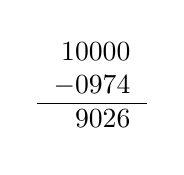
\begin{tikzpicture}
\draw(0,0)node{$
\begin{tabular}{r}
$10000$\\
$-0974$\\
\hline
$9026$
\end{tabular}
$};
\end{tikzpicture}
\end{otherlanguage}
\end{center}
\انتہا{مثال}
\ابتدا{مثال}
تکملہ \عددی{10}  کی مدد سے \عددی{974-7852}   حاصل کریں۔ 

\ترچھا{جواب}:\quad 
عدد \عددی{7852}   کے  اساسی تکملہ   \عددی{10000-7852=2148}   کا    \عددی{0974} کے ساتھ  مجموعہ     لیتے ہوئے: \عددی{0974+2148=3122}   آخری حاصل \عددی{1}  نہیں    پیدا ہوتا، لہٰذا یہ مجموعہ 
  \عددی{4}  ہندسوں پر مشتمل ہے؛  اس کے اساسی تکملہ \عددی{10000-3122=6878}   کے ساتھ منفی  علامت چسپاں کرتے ہوئے \عددی{-6878} کو جواب تسلیم کرتے ہیں۔
\begin{center}
\begin{otherlanguage}{english}
\begin{tikzpicture}
\draw(0,0.5)node[above,yshift=2em]{جواب}node[above,yshift=1em]{$-6878$};
\end{tikzpicture}\quad\quad
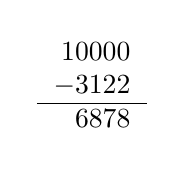
\begin{tikzpicture}
%\draw[thick,black] (-1,-1) grid (1,1);
%\draw [thin, gray,step=0.1](-1,-1) grid (1,1);
\draw(0,0)node{$
\begin{tabular}{r}
$10000$\\
$-3122$\\
\hline
$6878$
\end{tabular}
$};
\end{tikzpicture}\quad\quad
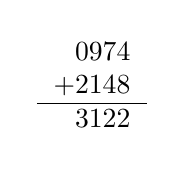
\begin{tikzpicture}
\draw(0,0)node{$
\begin{tabular}{r}
$0974$\\
$+2148$\\
\hline
$3122$
\end{tabular}
$};
\end{tikzpicture}\quad\quad
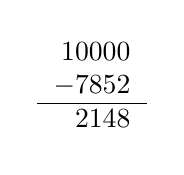
\begin{tikzpicture}
\draw(0,0)node{$
\begin{tabular}{r}
$10000$\\
$-7852$\\
\hline
$2148$
\end{tabular}
$};
\end{tikzpicture}
\end{otherlanguage}
\end{center}
\انتہا{مثال}

ثنائی اعداد بھی بالکل اسی طرح منفی کیے جاتے ہیں۔ان کی بھی دو مثالیں پیش کرتے ہیں۔
	

\ابتدا{مثال}
 اساسی تکملہ کی مدد سے مندرجہ ذیل حاصل کریں۔
 
(ا) \عددی{1011_2-11001_2} اور (ب) \عددی{11001_2-1011_2}

\ترچھا{جواب}:\quad
(ا) چونکہ \عددی{\overline{11001}=00110} ہے،   لہٰذا  تکملہ  دو  \عددی{00110+1=00111} ہو گا۔ اس کو  دوسرے عدد \عددی{01011_2}  (جس کی بائیں جانب  اضافی \عددی{0} چسپاں کر کے   ہندسوں کی  تعداد  پوری کی گئی) کے ساتھ جمع کرتے ہیں۔
\begin{align*}
\begin{split}
01011&\\
+00111&\\
\noalign{\smallskip}\hline\noalign{\smallskip}
10010&
\end{split}
\end{align*}
بائیں آخری  ہندسوں کو جمع کرتے ہوئے  حاصل  \عددی{1}  پیدا نہیں ہوا،  لہٰذا اس کا  تکملہ \عددی{2}  لینا ہوگا۔چونکہ  \عددی{\overline{10010}=01101} ہے لہٰذا اساسی تکملہ \عددی{01101+1=01110} ہو گا، جس کی  بائیں جانب منفی  علامت چسپاں کر کے  نتیجہ  \عددی{-01110_2} حاصل کرتے ہیں۔

\ترچھا{جواب}:\quad  (ب) یہاں ایک عدد پانچ ہندسوں پر مشتمل  ہے،  لہٰذا دوسرے عدد  میں بھی  پانچ ہندسے پورے  کیے  جائیں گے۔یوں \عددی{1011}   کو \عددی{01011} لکھ کر،  اس  کے   متمم 
 \عددی{\overline{01011}=10100} سے  عدد کا اساسی تکملہ \عددی{10100+1=10101} حاصل کر  کے،  دوسرے عدد کے ساتھ جمع کرتے ہیں۔
\begin{align*}
\begin{split}
1\phantom{11001}&\\
11001&\\
+10101&\\
\noalign{\smallskip}\hline\noalign{\smallskip}
101110&
\end{split}
\end{align*}
آخری ہندسے جمع کرتے ہوئے حاصل \عددی{1} پیدا ہوا جس کو نظرانداز کرکے  باقی مجموعہ \عددی{01110_2} کو نتیجہ  تسلیم کرتے  ہیں۔
\انتہا{مثال}
%????KKKKK

\حصہ{دو اعداد کی منفی بذریعہ اساس منفی ایک   تکملہ}
	اساس-منفی-ایک کے تکملہ کی مدد سے بھی دو اعداد منفی کئے جا سکتے ہیں۔مندرجہ ذیل اقدام پر چلنے سے یوں  حاصل کیا جاسکتا ہے۔

    • دونوں اعداد میں ہندسوں کی تعداد برابر ہونی چاہیے لہٰذا کم ہندسوں پر مبنی عدد کے بائیں جانب صفریں لگا کر اس میں ہندسوں کی تعداد دوسرے عدد جتنا کریں۔فرض کریں کہ یوں دونوں اعداد میں  ہندسے ہو جاتے ہیں۔
    •  کے ساتھ  کا اساس-منفی-ایک کا تکملہ جمع کریں 
      یعنی حاصل کریں۔
    • اگر  کی قیمت  کی قیمت سے زیادہ ہو تب جواب میں بائیں جانب 1 حاصل ہو گا اور یوں جواب  ہندسوں پر مبنی ہوگا۔اس صورت میں بائیں جانب حاصل 1 کو نظر انداز کرنے کی بجائے اس کو باقی عدد سے علیحدہ کر کے اس کا وزن اکائی تصور کریں اور پھر  اسے بقایا ہندسوں پر مبنی عدد کے ساتھ جمع کرکے جواب حاصل کریں۔اس کو واپسیں آخری حاصل ایک کہتے ہیں۔
    • اگر کی قیمت کی قیمت سے کم ہو تب کا جوابہندسوں پر مبنی ہوگا اور یہ ایک منفی عدد کو ظاہر کرے گا۔اس صورت میں حاصل جواب کا اساس-منفی-ایک کا تکملہ لے کر اس کے ساتھ نفی کا نشان لگائیں۔یہ اصل جواب ہو گا۔
یہ دونوں صورتیں مثالوں سے واضح ہوں گی۔
مثال 2.4: تکملہ-9 استعمال کرتے ہوئے   حاصل کریں۔ 

جواب: شکل 2.5 سے رجوع کریں۔
  کا تکملہ-9  ہے۔
اس  کا تکملہ-9  کو  کے ساتھ جمع کرکے حاصل ہوتا ہے۔یہ عدد چار ہندسوں پر مبنی ہے لہٰذا اس کا  تکملہ-9 لیتے ہیں۔۔اس تکملہ کے ساتھ نفی کا نشان جوڑ کر جواب ملتا ہے یعنی جواب ہے۔

مثال 2.5: تکملہ-9 استعمال کرتے ہوئے   حاصل کریں۔ 

جواب: شکل 2.6 سے رجوع کریں۔
  کا تکملہ-9  ہے۔
تکملہ-9  کو  کے ساتھ جمع کر کے حاصل ہوتا ہے۔یہ عدد پانچ ہندسوں پر مبنی ہے لہٰذا بائیں جانب ایک کو عدد سے علیحدہ کر کے اسے اکائی تصور کرتے ہوئے بقایا عدد کے ساتھ جمع کرکے جواب حاصل کرتے ہیں


	اب ہم ثنائی اعداد کی مثال لیتے ہیں۔

مثال 2.6: مندرجہ ذیل سوال کو تکملہ-1  کی مدد سے حل کریں
(ا) 
(ب) 

حل (ا):

لہٰذا
 
آخری حاصل ایک کو باقی عدد سے علیحدہ کر کے اسے اکائی  کی جگہ جمع کرتے ہوئے

جواب حاصل ہوتا ہے 

حل (ب):

لہٰذا

چونکہ بائیں جانب آخری حاصل صفر ہے لہٰذا جواب حاصل کرنے کے لئے اس  کا تکملہ-1 لیکر اس کے ساتھ نفی کا نشان لگاتے ہیں۔چونکہ

لہٰذا جواب ہے
 
2.7 مثبت اور منفی اعداد
	عام زندگی میں مثبت اعداد لکھتے ہوئے ان کے ساتھ بائیں جانب  جمع کی علامت لگائی جاتی ہے یا پھر انہیں بغیر کسی علامت کے لکھا جاتا ہے البتہ منفی اعداد لکھتے ہوئے ان کے ساتھ نفی کی علامت ضرور لکھی جاتی ہے۔یوں مندرجہ ذیل اعداد لکھنے کے درست طریقے ہیں۔

 
(2.12)

	کسی بھی عدد کے مثبت یا منفی ہونے کو اس عدد کا سائن 9 کہتے ہیں۔ یوں وہ اعداد جو مثبت یا منفی سائن رکھتے ہوں کو بمع-سائن-اعداد 10 کہتے ہیں اور جن اعداد کا کوئی سائن  نہ ہو ان کو بغیر-سائن-اعداد 11 کہتے ہیں۔اعداد کو ان کے سائن  اور مقدار سے ظاہر کرنے کے طریقہ کو بمع-سائن-مقدار کا نظام 12 کہتے ہیں۔ 
	کمپیوٹر میں حسابی عمل ثنائی اعداد 13 پر مبنی ہے جس میں کل دو ہی علامتیں یعنی صفر اور ایک ہیں۔کمپیوٹر میں کسی بھی معلومات کو انہیں دو علامتوں کی مدد سے ظاہر کیا جاتا ہے۔روایتی طور پر مثبت یعنی + کی علامت کو صفر یعنی  سے اور نفی یعنی -  کی علامت کو ایک یعنی  سے ظاہر کیا جاتا ہے۔یہ علامت عدد کے بائیں جانب لکھی جاتی ہے۔شکل 2.7 میں اس کی وضاحت کی گئی ہے۔
	یہاں ایک دلچسپ بات سامنے آتی ہے۔اگر ہم شکل میں اعداد کے بائیں جانب آخری ہندسے کو علامت سمجھیں تب  کا مطلب بنتا ہے لیکن اگر ہم کو چار ثنائی ہنسوں کا عدد سمجھیں تب یہ یا کو ظاہر کرتا ہے۔

	اس صورتِ حال کو سمجھنا ضروری ہے کہ کیا ثنائی اعداد میں بائیں جانب آخری مقام پر صفر  یا ایک  اس عدد کے علامت کو ظاہر کرتا ہے یا یہ عدد کا حصہ ہے۔ اس کا فیصلہ ان اعداد کو استعمال کرنے والے پر منحصر ہے۔کمپیوٹر استعمال کرتے وقت آپ خود یہ فیصلہ کرتے ہیں کہ آیا آپ سائن  رکھنے والے اعداد استعمال کریں گے یا بغیر سائن والے اعداد۔جدول 2.1 میں چار ثنائی ہندسوں پر مشتمل ممکنہ تمام اعداد دئے گئے ہیں۔
بمع-سائن-مقدار
ثنائی اعداد
































جدول 2.1:

	شکل میں کل چار ثنائی ہندسے  لکھائی کے لئے استعمال کئے گئے ہیں۔کمپیوٹر میں اعداد کو عموماً ایک بائٹ کی مدد سے لکھا جاتا ہے جس میں ہندسے ہوتے ہیں۔ایک بائٹ استعمال کرتے ہوئے سائن رکھنے والے اعداد میں نچلے سات مقام، عدد کی مقدار لکھنے کے لئے استعمال کئے جاتے ہیں جبکہ بائیں جانب آخری مقام میں صفر یا ایک اس عدد کی مثبت یا منفی ہونے کو ظاہر کرتا ہے۔مساوات 2.13 میں اس طرح کے چند مثالیں دی گئی ہیں۔

 
(2.13)

	اس مساوات میں ایک دلچسپ بات سامنے آتی ہے۔اس طریقہ لکھائی میں صفر دو مختلف علامتیں رکھتا ہے۔منفی صفر اور مثبت صفر دونوں ممکن ہیں۔عام زندگی میں صفر مثبت ہی تصور کیا جاتا ہے۔
	اتنا کچھ کہنے کے بعد آپ کو بتاتا چلوں کہ کمپیوٹر میں نفی اعداد کو بمع-سائن-مقدار کے نظام میں نہیں بلکہ ان کو بمع-سائن-تکملہ-1 کے نظام یا بمع-سائن-تکملہ-2  کے نظام میں رکھا اور استعمال کیا جاتا ہے۔اگلے حصہ میں انہی نظاموں پر غور ہو گا۔
2.8 بمع-سائن-تکملہ کے نظام
	کمپیوٹر میں عددی الیکٹرانکس کی مدد سے اعداد کو جمع یا منفی کیا جاتا ہے۔ دیکھا یہ گیا ہے کہ یہ اعمال اس وقت زیادہ آسانی سے سرانجام دیئے جا سکتے ہیں جب اساسی تکملہ یا اساس-منفی-ایک کا تکملہ زیرِ استعمال لائے جائیں جیسا کہ کتاب کے حصہ 2.4 اور 2.5 میں دکھایا گیا ہے۔
	اسی بناء پر کمپیوٹر کی دنیا میں منفی اعداد کو اساسی تکملہ یا اساس-منفی-ایک کی تکملہ کی صورت میں ہی لکھا جاتا ہے۔کمپیوٹر ثنائی اعداد استعمال کرتا ہے لہٰذا اس میں منفی اعداد کو تکملہ-1 یا تکملہ-2 کی صورت میں لکھا جاتا ہے۔چار ثنائی ہندسوں پر مبنی تمام ممکنہ اعداد کو بمع-سائن تکملہ کی شکل میں جدول 2.2 میں دکھایا گیا ہے۔اسی میں انہیں بمع-سائن مقدار کے طور بھی دکھایا گیا ہے۔
بمع-سائن تکملہ-دو
بمع-سائن تکملہ-ایک
بمع-سائن مقدار
اعشاری اعداد
































نہیں پایا جاتا
























 






 
نہیں پایا جاتا
نہیں پایا جاتا

جدول 2.2:

	جدول 2.2 سے آپ دیکھ سکتے ہیں کہ کسی بھی مثبت عدد کو ثنائی ہندسوں میں ایک ہی طریقہ سے لکھا جاتا ہے جبکہ کسی بھی منفی عدد کو تین طریقوں سے لکھا جاتا ہے۔اس کا مطلب ہے کہ مثبت عدد کو ان تین طریقوں میں لکھنے کی خاطر اس عدد کو سادہ ثنائی عدد کی شکل میں لکھ دیں۔ 
	مثبت عدد  کو بمع-سائن شکل میں لکھ کر اس کے سائن کو صفر  سے تبدیل کر کے ایک  کرنے سے یعنی بمع-سائن منفی عدد حاصل ہوتا ہے۔یوں کو بمع-سائن عدد کی شکل میں لکھنے کی خاطر کو بمع-سائن عدد کی شکل میں لکھیں یعنی اور اس میں سائن کو صفر سے تبدیل کر کے ایک کر دیں یعنی ۔یہ کو بمع-سائن عدد کے طور لکھنے کا طریقہ ہے۔
	منفی عددکو بمع-سائن تکملہ-ایک کی صورت میں لکھنے کی خاطرکو بمع-سائن ثنائی عدد کے طور لکھیں (یعنی اس عدد کو سادہ ثنائی طریقہ سے لکھیں)۔اس ثنائی عدد کا تکملہ-1 حاصل کرنے سےکی بمع-سائن تکملہ-1 شکل حاصل ہوگی۔یاد رہے کہ تکملہ-1 حاصل کرتے وقت ثنائی عدد کے ہر ہندسے کو (بمع سائن کے)  اُلٹ کرنا ہوگا۔یوں کو بمع-سائن تکملہ-1 کی صورت میں لکھنے کی خاطر پہلے کو لکھیں اور پھر اس پورے چار ہندسوں پر مبنی عدد کو ایک عدد سمجھتے ہوئے اس کا تکملہ-1 لیں یعنی ۔یہیکو بمع-سائن تکملہ-1 میں ظاہر کرتا ہے۔
	منفی عددکو بمع-سائن تکملہ-دو کی صورت میں لکھنے کی خاطر اسے ثنائی عدد کے طور لکھ کر اس کا تکملہ-دو حاصل کریں۔مثلاً کو لکھیں اور اب ان چار ہندسوں پر مبنی عدد کا تکملہ-2 لیں یعنی ۔یہ کو بمع-سائن تکملہ-2 میں لکھنے کا طریقہ ہے۔
